% Compact editorial revision, 1 October 2026.
% The default is a two-column reading copy. For one-column review layout,
% compile submission.tex, which defines \reviewversion before reading this file.
% Scientific inputs are from the supplied manuscript; no inventory run is implied.
\ifdefined\reviewversion
\documentclass[essd,manuscript]{copernicus}
\else
\documentclass[essd]{copernicus}
\fi

% siunitx and the shared gas/unit shorthand, on the same terms as paper_national.tex: the
% class loads its own fontenc/inputenc, graphicx, amsmath, natbib, hyperref, tabularx,
% multirow, float and caption, and loading any of them again with other options is what
% breaks a Copernicus build. siunitx must precede the macros (\DeclareSIUnit), and the
% class defines a robust \unit that siunitx v3 refuses to define over, so the class's copy
% is released first - nothing here uses it.
%
% These are not cosmetic. Every printed quantity in this repository is checked against the
% product it came from, and the sweep that does it reads siunitx arguments and tabular
% cells. A number typed as bare prose is invisible to it: this file stated 85 quantities
% and the guard could see none of them, which is the same notation blindness the citation
% audit had when it read one of the two ways a filename gets written.
\let\unit\relax
\usepackage{siunitx}
\usepackage{placeins} % v3: every figure is placed before the conclusions (FloatBarrier below), so none lands after the references in the one-column submission build
% ===========================================================================
% paper_common/macros.tex - the shorthand every manuscript shares.
%
% Split from preamble.tex in the ESSD re-targeting: the national article now compiles
% under the Copernicus class, which loads its own packages and forbids most of what
% preamble.tex sets (geometry-like options, a second hyperref, placeins), but it needs
% exactly the same shorthand as the sector reports. The macros therefore live here, on
% their own, and preamble.tex inputs this file so that every other manuscript keeps
% compiling unchanged. A macro that renders differently in two documents is the defect
% this file exists to prevent; define it once.
%
% Requires: siunitx (for \DeclareSIUnit and \si) - the caller loads it.
% ===========================================================================

% Gas and pollutant names.
\newcommand{\COtwo}{CO\textsubscript{2}}
\newcommand{\COe}{CO\textsubscript{2}e}
\newcommand{\CHfour}{CH\textsubscript{4}}
\newcommand{\NtwoO}{N\textsubscript{2}O}
\newcommand{\NHthree}{NH\textsubscript{3}}
\newcommand{\NOx}{NO\textsubscript{x}}
\newcommand{\SOtwo}{SO\textsubscript{2}}
\newcommand{\PM}{PM\textsubscript{2.5}}
\newcommand{\MCF}{MCF}
\newcommand{\Mt}{\text{Mt~\COe}}
\newcommand{\tCha}{\si{\tonne\per\hectare}}
\newcommand{\AFOLU}{AFOLU}
\newcommand{\GLW}{GLW\,4}
\newcommand{\EFone}{EF\textsubscript{1}}

% siunitx: allow Mt, Tg, ha, head, yr, dB
\DeclareSIUnit{\head}{head}
\DeclareSIUnit{\yr}{yr}
\DeclareSIUnit{\dB}{dB}

% A file name is the one long unbreakable token these documents are full of -
% \texttt{waste\_air\_pollutants\_2024.csv} is wider than a two-column measure and TeX prints
% it past the margin rather than breaking it. Allowing a break AFTER each escaped underscore
% costs nothing and inserts no hyphen, which matters: a hyphenated file name is a wrong file
% name. This is one line because every such name in every document is written with \_.
\let\pkinvunderscore\_
\renewcommand{\_}{\pkinvunderscore\allowbreak}


\begin{document}
% Compact front matter; insert after \begin{document} in the official class.
% Dataset DOI and release version remain pending in the availability statement.
\title{PakEmis: a national greenhouse gas emissions inventory for Pakistan, July 2015--June 2024}
\Author[1][rehan@pakairquality.com]{Rehan}{Ahmad}
\affil[1]{Pakistan Air Quality Initiative (PAQI), Karachi, Pakistan}
\runningtitle{A greenhouse gas emissions inventory for Pakistan}
\runningauthor{R. Ahmad}
\received{}
\pubdiscuss{}
\revised{}
\accepted{}
\published{}
\firstpage{1}
\maketitle

\begin{abstract}
Pakistan's greenhouse gas emissions are estimated from activity records kept by different institutions at different levels of detail, and these records cannot always be combined directly. We present PakEmis, a national inventory of CO$_2$, CH$_4$ and N$_2$O outside land use, land-use change and forestry, covering nine fiscal years from July 2015 to June 2024. The inventory compiles Pakistani regulatory, statistical, survey and operator records, reconciles the fuel and biomass quantities that sectors share, and applies IPCC methods with Pakistani activity statistics. Annual estimates are linked to monthly profiles and a \SI{0.05}{\degree} grid, and to provincial and district tables, with the evidence behind each allocation recorded. Under the reference assumptions, the estimated categories total \SI{451.86}{\mega\tonne}\,CO$_2$e in 2023--24 using IPCC Fifth Assessment Report 100-year global warming potentials, with a conditional \SI{95}{\percent} Monte Carlo interval of \SIrange{406.71}{532.86}{\mega\tonne}\,CO$_2$e, and the estimate rises by \SI{50.96}{\mega\tonne} over the period. Using household-survey dung consumption instead of agriculture-derived diversion gives \SI{446.73}{\mega\tonne}\,CO$_2$e, and alternative readings of the public-power coal account move the total between \SI{450.27}{} and \SI{469.64}{\mega\tonne}\,CO$_2$e; these alternatives are reported beside the parameter interval rather than inside it. Monthly allocation is limited by the available records: \SI{54.18}{\percent} of reference-year emissions use flat or weakly constrained profiles. Fluorinated gases, several industrial sources and industrial wastewater are not estimated. The dataset identifier and citation are given in the data availability section.
\end{abstract}

\introduction
\label{sec:introduction}

Pakistan's greenhouse gas emissions are estimated from activities recorded by different institutions and at different levels of detail. Fuel accounts describe energy supply and consumption, agricultural statistics describe livestock and crop production, and household surveys provide information on domestic fuel use. These records offer a basis for a national inventory, but they cannot always be combined directly.

Four difficulties recur. A fuel account describes fuel supplied to a customer class, while an inventory needs the fuel burned by a source: the regulator's aggregate coal energy for public power, for example, implies more coal than the country imported and produced, whereas the stations' own metered tonnage does not (Sect.~\ref{sec:validation}). Quantities overlap: gas that leaks from the network is also counted in delivered gas, petrol sold to the road customer class also fuels household generators, and dung removed from manure management is burned as household fuel. Reporting periods differ: energy statistics follow the July--June fiscal year, livestock statistics and international comparators follow the calendar year, and household surveys describe a survey round. Geographical information is uneven: a fuel account constrains national combustion without saying where the fuel was burned, and monthly sales can precede consumption.

Pakistan's official reporting provides the national context. The First Biennial Update Report includes an inventory for FY2017--18, and the Biennial Transparency Report provides a category-level inventory for FY2020--21, and the associated Common Reporting Tables report calendar year 2022 \citep{PakistanBUR2022,PakistanBTR2024,PakistanCRT2026}. These submissions also identify coverage gaps that affect comparisons: residential biomass, for example, is reported as not estimated in the Common Reporting Tables, so two residential totals can differ because of the fuels included even when the estimates for the fuels common to both agree. International inventories add further estimates: EDGAR covers most sectors, FAOSTAT provides agricultural emissions, and Climate TRACE combines sectoral and asset-level information \citep{EDGAR2025,FAOSTAT2025,Tubiello2013,ClimateTRACE2026}. These products differ in method and source boundary, and they can share activity statistics or emission factors with a national estimate, so agreement between two totals may reflect common inputs rather than independent confirmation.

PakEmis addresses these difficulties through the work it performs on the records. We compile the regulatory, statistical, survey and operator records into activity tables that retain their original period, units and source; we reconcile the quantities that sectors share so that each is used once; we estimate CO$_2$, CH$_4$ and N$_2$O with IPCC methods \citep{IPCC2006,IPCC2019}; and we allocate the annual estimates to months, administrative areas and a \SI{0.05}{\degree} grid while recording the evidence each allocation rests on. Where the records support more than one reading of a quantity, as they do for public-power coal energy and for household dung, we report the alternatives beside the reference calculation rather than selecting one silently. Categories that cannot be estimated and emissions that cannot be placed remain identified as such.

The paper describes the source records and methods (Sect.~\ref{sec:methods}), reports the inventory and its sensitivity to the readings of the evidence (Sect.~\ref{sec:results}), evaluates it against internal checks and external inventories (Sect.~\ref{sec:validation}), and describes the products and their recommended use (Sect.~\ref{sec:use}).

\section{Data and methods}
\label{sec:methods}

\subsection{Scope and source records}
\label{sec:scope}

The inventory covers nine fiscal years from July 2015 to June 2024. Each fiscal year runs from July to June; 2023--24 is the reference year, for which the monthly grid and the uncertainty analysis are built. The inventory estimates CO$_2$, CH$_4$ and N$_2$O for agriculture, electricity generation, transport, residential fuel, industrial combustion, industrial processes and product use (IPPU), oil and gas fugitives, and waste. Land use, land-use change and forestry (LULUCF) are outside its scope. Fluorinated gases, coal-mining fugitives, industrial wastewater and several other industrial sources are not estimated; a category--gas matrix records these gaps separately from zeros and from emissions included elsewhere.

Activity comes from regulatory reports, agricultural and population statistics, household surveys, and operator records (Table~\ref{tab:sources}). Energy inputs come principally from the National Electric Power Regulatory Authority (NEPRA), the Hydrocarbon Development Institute of Pakistan (HDIP), the Oil and Gas Regulatory Authority (OGRA) and the Oil Companies Advisory Council (OCAC). The Pakistan Bureau of Statistics (PBS) supplies census, household and industrial data, and the National Fertilizer Development Centre (NFDC) supplies fertiliser records. Each compiled input retains its original period, units, source edition and conversion; the full source register and the sector-specific calculations are in the technical documentation.

\begin{table*}[t]
\caption{Principal source records. Editions are those held and transcribed; the full per-file register with page and table citations is \texttt{outputs/pakemis\_source\_register.csv}. Fuel energy is obtained from mass or volume at the IPCC 2006 net calorific value for the fuel or coal rank unless the row states another basis.}
\label{tab:sources}
\footnotesize
\begin{tabular}{@{}>{\raggedright\arraybackslash}p{3.1cm}>{\raggedright\arraybackslash}p{4.3cm}>{\raggedright\arraybackslash}p{2.6cm}>{\raggedright\arraybackslash}p{2.6cm}>{\raggedright\arraybackslash}p{3.6cm}@{}}
\tophline
Quantity & Publication and edition & Reporting period & Units as published & Conversion or use \\
\middlehline
Station fuel and generation & NEPRA State of Industry Report 2018, 2023 and 2024 (per-station tables) & 2015--16 to 2023--24 & tonnes, MMCFT, MMBTU; GWh & coal to TJ at the rank default; gas at the declared heating value \\
Coal by consumer; supply & Finance Division Economic Survey Statistical Supplement 2024--25 (Tables 14.1, 14.3); HDIP Energy Yearbook (Table 4.4) & fiscal years & kt; TOE & supply bound and consumer allocation (Sect.~\ref{sec:validation}) \\
Gas sales by sector & OGRA State of the Regulated Petroleum Industry, 2015--16 to 2023--24 editions & fiscal years & MMCFD, MMCF & delivered gas; leakage deducted before combustion \\
Petroleum sales by customer class & OCAC sectoral sales, annual (2016--17 onward) and monthly (July 2021 onward) & fiscal years; months & tonnes by product & road, off-road, generator and aviation partitions; monthly profiles \\
Livestock & PBS 7th Agricultural Census 2024; FAOSTAT historical stocks & 2024 enumeration; calendar years & head & Tier~1 factors; historical series on the calendar basis \\
Household fuel & PBS HIES 2018--19 and 2024--25 & survey rounds & kg per household per month, design-weighted & national firewood and dung-cake consumption \\
Fertiliser & NFDC Fertilizer Review 2023--24 (monthly offtake) & fiscal years; months & nutrient tonnes & managed soils and urea; monthly profile \\
Crops and residues & Pakistan Economic Survey 2023--24 agriculture appendix; PBS crop dashboard & fiscal years & tonnes; hectares & rice area-days, residue ledger \\
Industrial production & PBS Monthly Minerals Production and Quantum Index of Manufacturing & fiscal years; months & tonnes; index & cement, lime, steel; monthly profiles \\
Railways; aviation & Pakistan Railways operator records; PCAA Major Traffic Flows & fiscal years & thousand litres; movements & diesel combustion; domestic flights \\
Waste & PBS population census; World Bank What a Waste 2.0; JMP sanitation shares & census years; 2018; 2023 & persons; kg per person per day; shares & first-order decay; wastewater pathways \\
\bottomhline
\end{tabular}
\end{table*}

A fiscal-year label does not make every input a fiscal-year observation. Reference livestock numbers are the 2024 agricultural census enumeration; household fuel use is the adjacent HIES 2024--25 round; and the historical livestock series keeps its calendar-year basis \citep{PBSAgri2026,PBSHIES2026}. Crop production and fertiliser offtake are fiscal records. Approximately \SI{77}{\percent} of the reference agricultural estimate comes from enteric fermentation and manure management, so the historical livestock reconstruction affects the national series materially, and its annual values are not successive fiscal-year census observations.

\subsection{Emission estimates and shared material flows}
\label{sec:estimation}

For a source $s$, gas $g$ and year $y$, the basic estimate is
\begin{equation}
 E_{s,g,y}=A_{s,y}\,\mathrm{EF}_{s,g},
 \label{eq:annual}
\end{equation}
where $A$ is activity and EF is the corresponding emission factor. Most sources use Tier~1 methods from the IPCC Guidelines with Pakistani activity statistics and relevant updates from the 2019 Refinement \citep{IPCC2006,IPCC2019}. Fuel mass is converted to energy on the calorific basis its factor requires; livestock, soil and waste calculations use the animal, nitrogen or organic-carbon basis of their methods. Quantities are calculated by source and then aggregated to reporting categories.

We retain native-gas mass and apply global warming potentials (GWPs) at reporting. The headline AR5 100-year values are 1 for CO$_2$, 28 for biogenic CH$_4$, 30 for fossil CH$_4$ and 265 for N$_2$O \citep{IPCCAR5}; AR6 equivalents are provided separately \citep{IPCCAR6}. Biomass-combustion CO$_2$ is a memo item outside the total, while its CH$_4$ and N$_2$O are included, following inventory reporting conventions.

\paragraph{Public-power coal.} The reference public-power coal energy is calculated from each generating station's metered coal tonnage as reported in the regulator's station tables, converted at the IPCC 2006 net calorific value for the rank the station burns (lignite at the Thar stations, imported coal elsewhere) and summed over the enumerated stations. For the years before the per-station tables begin, the same account is reconstructed from the editions that print each station's mass or its generation and fuel intensity, with the two commissioning years carried as a bounded lane. Two other readings of the same quantity exist and are reported in Sect.~\ref{sec:sensitivity}: the aggregate coal energy the regulator publishes as ``fuel consumed'', which on the fleet's rank composition implies more coal than the country supplied in 2023--24 (Sect.~\ref{sec:validation}), and the energy implied by each station's own heat rate and generation, which is derived from generation and therefore cannot test it. Captive industrial generation is estimated separately and contributes to industrial combustion.

Combustion estimates combine fuel records with the factors for each use. Industrial fuels include metered gas, petroleum products and recorded coal use in brick kilns and cement production. Road and off-road estimates partition the petroleum customer classes; railway fuel comes from operator records; aviation covers domestic activity. Household electricity is excluded at the point of consumption because generation emissions are already included. IPPU covers cement, ammonia, iron and steel, and lubricant use, with process carbon separated from the fuel burned to operate the plants.

Agricultural estimates cover enteric fermentation, manure management, managed soils, rice, residue burning and urea application. Livestock populations and per-head factors determine enteric methane. Excreted nitrogen is partitioned among grazing, manure management and fuel diversion, with management losses deducted before soil application; direct and indirect soil N$_2$O are then calculated from the nitrogen reaching each pathway. The reference direct factor for non-rice cropland is the dry-climate value of \num{0.005}~kg N$_2$O--N per kilogram of nitrogen; flooded rice and grazing use separate factors. Rice methane depends on cultivated area, cultivation duration and water management. Crop residues are divided among soil return, field burning, fuel and other destinations before emissions are assigned.

Residential fuels combine domestic sales with weighted HIES quantities. Dung connects the household account to the agricultural manure calculation, and the two records disagree: the agricultural diversion implies \SI{58.74}{\mega\tonne} of air-dry dung cake, whereas the survey estimate of household demand is \SI{11.97}{\mega\tonne}. Configuration L assigns the diverted quantity to households; configuration S uses household demand and leaves approximately \SI{46.8}{\mega\tonne} with other or unresolved destinations. Balancing the agricultural diversion establishes how much dung left manure management; it does not establish how much households burned, which is why the two readings are carried separately with no probabilities assigned.

Waste estimates use urban and rural population, generation rates, collection shares and treatment pathways. Solid-waste methane follows first-order decay of historical deposits with a deposit history extending to 1960, so each year's estimate depends on the deposits accumulated to that year. Open burning is applied to a share of uncollected waste, and the unburned remainder retains an unresolved fate. Domestic wastewater methane follows organic load and sanitation pathways; N$_2$O is calculated from nitrogen in effluent. Historical generation, collection and sanitation parameters are held fixed, so the waste series principally reflects demographic change and accumulated deposits.

Oil and gas fugitives are estimated by production, processing, transmission and distribution segment from throughput and infrastructure records; operating practice and coverage remain uncertain and are carried as separate configurations. Gas assigned to leakage is deducted from the delivered gas used in combustion. Other shared quantities are handled in the same way: petrol assigned to residential generators is deducted from the customer-class quantity otherwise used for road transport, dung removed from manure management enters the fuel balance, and retail diesel is partitioned between road and off-road use. These deductions prevent a quantity from being counted twice; the activity and destination assumptions behind them are evaluated in Sect.~\ref{sec:validation}.

\subsection{Monthly and spatial products}
\label{sec:allocation}

Monthly and spatial estimates are derived from the annual source estimates. Monthly profiles distribute emissions through the year, while spatial weights assign them to supported locations. Emissions without sufficient location information remain unallocated. For a monthly profile $p$ and spatial weight $w$,
\begin{equation}
\begin{aligned}
 E_{s,g,y,m,i}&=E_{s,g,y}\,p_{s,y,m}\,w_{s,y,i},\\
 \sum_m p_{s,y,m}&=1,\qquad \sum_i w_{s,y,i}=1,
\end{aligned}
 \label{eq:allocation}
\end{equation}
for the streams that can be placed (Fig.~\ref{fig:construction}). The spatial weight carries no month index: within a year the spatial pattern of a stream is fixed and its months differ in magnitude only, which is how the products are built. A national total reconstructed from the products therefore includes both the placed and the unallocated mass. The reference monthly grid combines timing and location; the historical grids are annual.

Temporal profiles use plant dispatch, petroleum sales, fertiliser offtake, industrial production, fire detections or process assumptions, depending on the source. Each stream-year is assigned one of four evidence classes: observed source-month activity (class TE1), reconstructed monthly administrative activity (TE2), a process or activity-shape profile (TE3), or a flat or weakly constrained profile (TE4). A flat profile assumes a constant daily rate and weights months by their length, including leap days; it expresses unresolved seasonality rather than an observation. Sales and production profiles keep their own meaning: fertiliser offtake, for example, precedes application and the soil emissions that follow.

Spatial products use a fixed \SI{0.05}{\degree} grid. Facilities are placed at supported locations; distributed sources use administrative activity or proxies such as crop, livestock, settlement and infrastructure patterns. Administrative summaries use a \num{152}-unit district frame based on geoBoundaries 2019. Historical weights are taken from the same year where a record supports them; otherwise the weight is a timeless structural surface, the reference year's pattern rescaled, or a declared substitute, and the class is recorded for every stream-year. The maps therefore combine annual changes in the source estimates with spatial evidence of varying age.

The units are chosen for reuse. Gridded values are native-gas mass per cell and period, not flux density; conversion to kg~m$^{-2}$~s$^{-1}$ requires the cell area and the period duration. Country fractions must be handled consistently with the allocation, and the unallocated mass must be retained when reproducing a national total. Administrative and gridded views describe the same inventory and must not be added together.

\begin{figure*}[t]
\centering
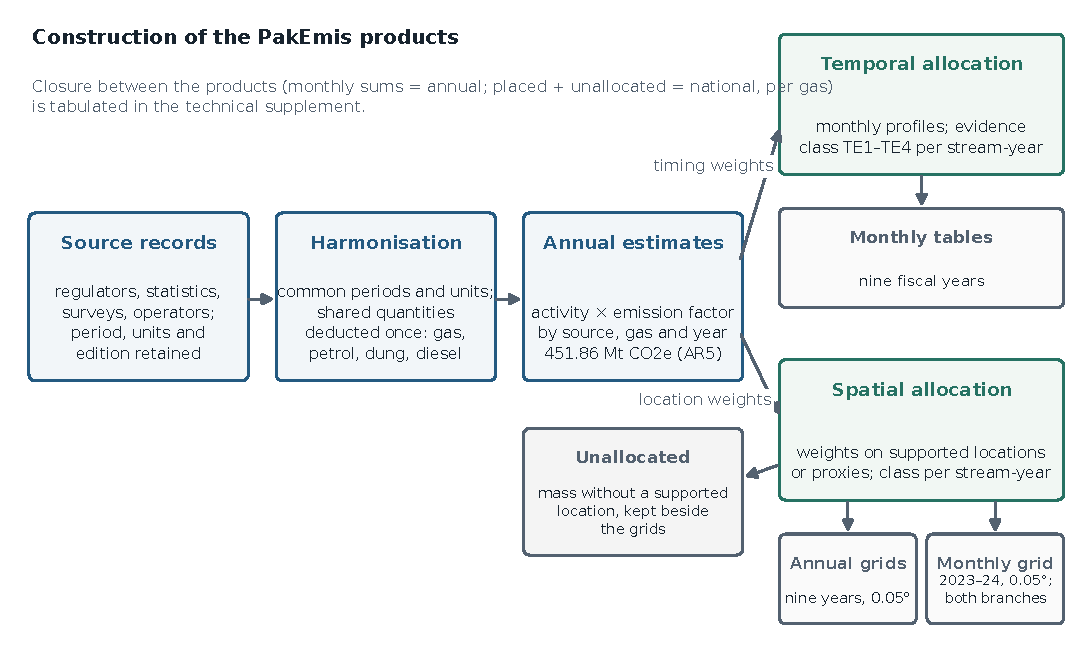
\includegraphics[width=\textwidth,height=0.72\textheight,keepaspectratio]{../../figures/fig1_data_products.pdf}
\caption{Construction of the data products. Source records are harmonised into activity tables, from which annual estimates are made by source and gas; temporal and spatial allocation then proceed as parallel branches to the monthly tables and the annual and monthly grids, with emissions that lack a supported location retained in the unallocated account on the spatial branch. The closure identities between the products are tabulated in the technical documentation.}
\label{fig:construction}
\end{figure*}

\subsection{Uncertainty and evaluation}
\label{sec:uncertainty}

Three kinds of uncertainty are kept apart, because they answer different questions:
\begin{enumerate}
\item parameter uncertainty within the selected configuration --- activity, emission factors and conversion factors, sampled with their stated distributions;
\item alternative interpretations of the source evidence --- the public-power coal account, household dung use, sewer conditions and fugitive practice, each reported as a named configuration with no probability assigned;
\item unestimated categories and allocation limitations --- recorded in the category--gas matrix and in the evidence class of every placement.
\end{enumerate}
The national parameter interval describes the first of these only.

A \num{100000}-realization Monte Carlo calculation samples the parameters and combines them with the waste and fugitive sectors' own distributions. Shared inputs receive the same draw wherever they enter the account. Two settings test fuel-carbon factors shared only within a calculation module or across all combustion modules. National percentiles are taken after summing each realization. A common subset of realizations supports the monthly and provincial products, which remain conditional on their selected allocation. Distributions, seeds, dependence groups and the registry-based sensitivity analysis are described in the technical documentation.

Changes over time are calculated from paired realisations because errors shared between years can cancel in their difference. The reference dependence setting holds persistent parameters, such as emission factors, fixed across years while annual activity varies; a fully time-correlated setting and a time-independent setting bound the sensitivity to that choice.

Evaluation examines magnitude, timing and location. Internal tests check the shared-quantity deductions, gas aggregation and conservation across the products. External comparisons state the benchmark version, period, source boundary, gas and reporting metric; we compare native-gas mass where it is available, align GWPs for CO$_2$ equivalents, and keep fiscal--calendar offsets visible, since an average of adjacent calendar years only approximates a fiscal year. Shared statistics and factors are identified for each comparison.

\section{Inventory results}
\label{sec:results}

\subsection{Composition and historical change}
\label{sec:composition}

Estimated emissions total \SI{451.86}{\mega\tonne}~CO$_2$e in 2023--24 under configuration L and AR5 GWPs. By calculation module, agriculture contributes \SI{223.45}{\mega\tonne}, the power module \SI{45.59}{\mega\tonne}, transport \SI{41.93}{\mega\tonne} and waste \SI{37.91}{\mega\tonne} (Fig.~\ref{fig:inventory}a). These modules are groups of calculations, not IPCC reporting sectors: the power module includes captive industrial generation, which IPCC reporting assigns to industrial combustion, and transport includes off-road machinery. The category--gas account under IPCC codes is given in the technical documentation.

Methane contributes \SI{248.78}{\mega\tonne}~CO$_2$e, \SI{55.1}{\percent} of the total; CO$_2$ and N$_2$O contribute \SI{160.94}{} and \SI{42.13}{\mega\tonne}~CO$_2$e. Enteric fermentation is the largest category at \SI{151.66}{\mega\tonne}, \SI{33.6}{\percent} of the inventory, which is why livestock populations and emission factors govern both the total and its uncertainty. Reporting the same native-gas emissions with AR6 GWPs gives \SI{444.95}{\mega\tonne}~CO$_2$e; the \SI{6.91}{\mega\tonne} difference is a change of metric, not of emissions.

The historical estimate rises from \SI{400.90}{\mega\tonne} in 2015--16 to \SI{451.86}{\mega\tonne} in 2023--24 (Fig.~\ref{fig:inventory}b). The trajectory is uneven: it peaks at \SI{490.58}{\mega\tonne} in 2020--21 and falls to \SI{445.24}{\mega\tonne} in 2022--23, and the peak's position is not robust, since 2021--22 is \SI{490.49}{\mega\tonne}, within \SI{0.1}{\mega\tonne} of it. Estimated emissions increase by \SI{50.96}{\mega\tonne}~CO$_2$e (\SI{12.7}{\percent}) over the study period. The conditional interval excludes zero under the reference and fully correlated parameter settings, but includes zero under time independence: the reference setting gives \SIrange{12.75}{93.01}{\mega\tonne}, the time-correlated setting \SIrange{39.96}{64.04}{\mega\tonne}, and the time-independent setting \SIrange{-12.48}{117.11}{\mega\tonne} (Fig.~\ref{fig:inventory}c). Individual year-to-year fluctuations also depend on reconstructed activity, principally the livestock series and the industrial coal allocation.

\begin{figure*}[t]
\centering
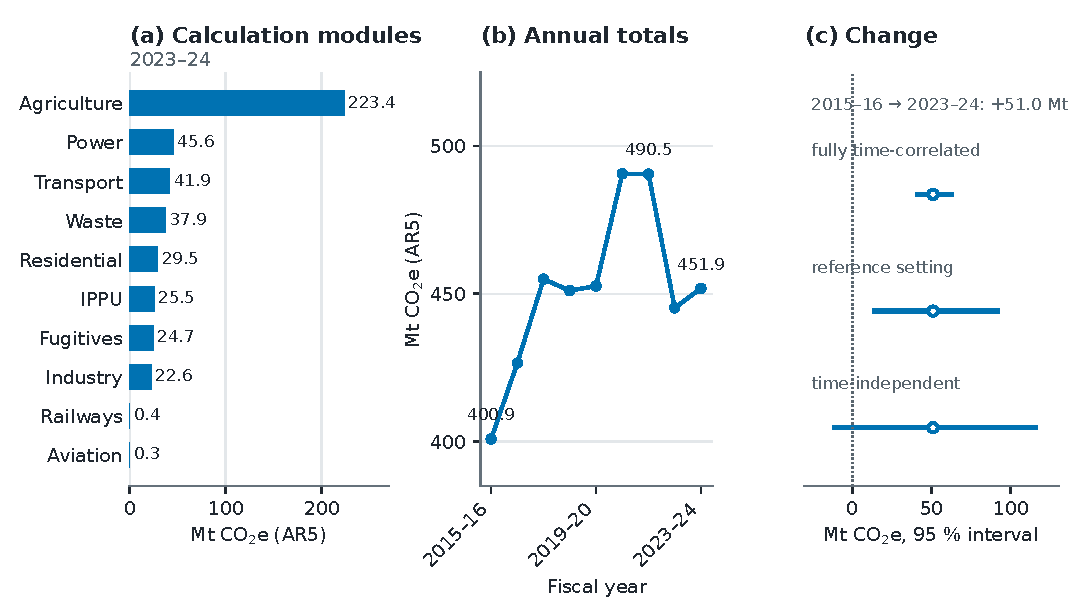
\includegraphics[width=\textwidth,height=0.72\textheight,keepaspectratio]{../../figures/fig2_inventory.pdf}
\caption{Estimated emissions under the reference configuration and AR5 GWPs. (a) Reference-year totals by calculation module; the power module includes captive generation and transport includes off-road machinery. (b) Annual totals over the common ten-module scope; no per-year uncertainty interval exists and none is drawn. (c) The change from 2015--16 to 2023--24 with its \SI{95}{\percent} interval under the three temporal-dependence settings, from paired realizations (\texttt{pakemis\_trend\_uncertainty.csv}).}
\label{fig:inventory}
\end{figure*}

\subsection{Uncertainty and allocation evidence}
\label{sec:evidence}

The deterministic reference estimate is \SI{451.86}{\mega\tonne}~CO$_2$e; the Monte Carlo median is \SI{456.41}{\mega\tonne}, with a conditional \SI{95}{\percent} interval of \SIrange{406.71}{532.86}{\mega\tonne} (Fig.~\ref{fig:evidence}), approximately \SI{-10.9}{\percent} and \SI{+16.8}{\percent} around the median. Sharing fuel-carbon factors across modules changes the interval only slightly, to \SIrange{406.65}{533.20}{\mega\tonne}; this applies to the tested factor uncertainties and dependence structure and does not imply that dependence is unimportant for other inputs or for changes over time. In the Approach~1 category screen, which assumes independence between categories, enteric fermentation accounts for \SI{58.0}{\percent} of variance and domestic wastewater for \SI{15.9}{\percent}.

The monthly product is less strongly constrained than the annual total. Observed source-month activity supports \SI{0.94}{\percent} of reference-year emissions, reconstructed administrative activity \SI{24.90}{\percent} and process profiles \SI{19.99}{\percent}, while \SI{54.18}{\percent} is flat or weakly constrained. Across the nine-year panel, observed and reconstructed monthly activity together support \SI{18.49}{\percent} and the flat share is \SI{60.38}{\percent}. Twelve monthly values therefore do not mean twelve observations, and monthly analysis should be confined to the streams whose class supports it.

The reference spatial calculation places \num{199} of \num{202} streams; three aviation cruise streams, approximately \SI{0.06}{\percent} of the total, remain unallocated below their supported administrative level. This measures allocation completeness (\SI{99.94}{\percent} of the mass is placed), not positional accuracy: most of the placed mass rides administrative shares or proxy surfaces, and by mass \SI{61.5}{\percent} of the reference year sits on a timeless structural surface, \SI{30.9}{\percent} on that year's observed activity and \SI{7.5}{\percent} on a declared substitute (\texttt{pakemis\_spatial\_basis\_shares.csv}). The reference-year grid itself is shown in Fig.~\ref{fig:grid} and the evidence behind its placement in Fig.~\ref{fig:grid_evidence}.

\begin{figure*}[t]
\centering
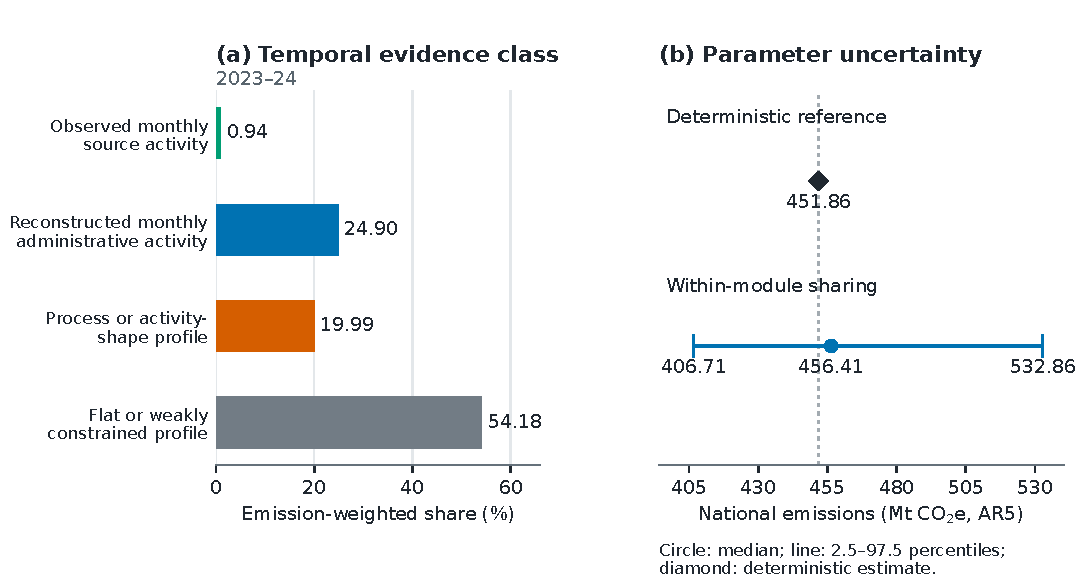
\includegraphics[width=\textwidth,height=0.72\textheight,keepaspectratio]{../../figures/fig3_evidence_uncertainty.pdf}
\caption{Evidence behind the monthly allocation and the national parameter interval. (a) Share of reference-year emissions by temporal evidence class: observed source-month activity, reconstructed monthly administrative activity, process or activity-shape profile, and flat or weakly constrained profile. (b) The conditional national \SI{95}{\percent} Monte Carlo interval under within-module parameter sharing, with the median and the deterministic reference estimate marked. Sharing fuel-carbon factors across modules moves the interval from \SIrange{406.71}{532.86}{\mega\tonne} to \SIrange{406.65}{533.20}{\mega\tonne}: \SI{-0.06}{\mega\tonne} at the lower endpoint and \SI{+0.34}{\mega\tonne} at the upper, on a width of \SI{126}{\mega\tonne}. The interval describes parameter uncertainty in annual magnitude only.}
\label{fig:evidence}
\end{figure*}

\begin{figure*}[t]
\centering
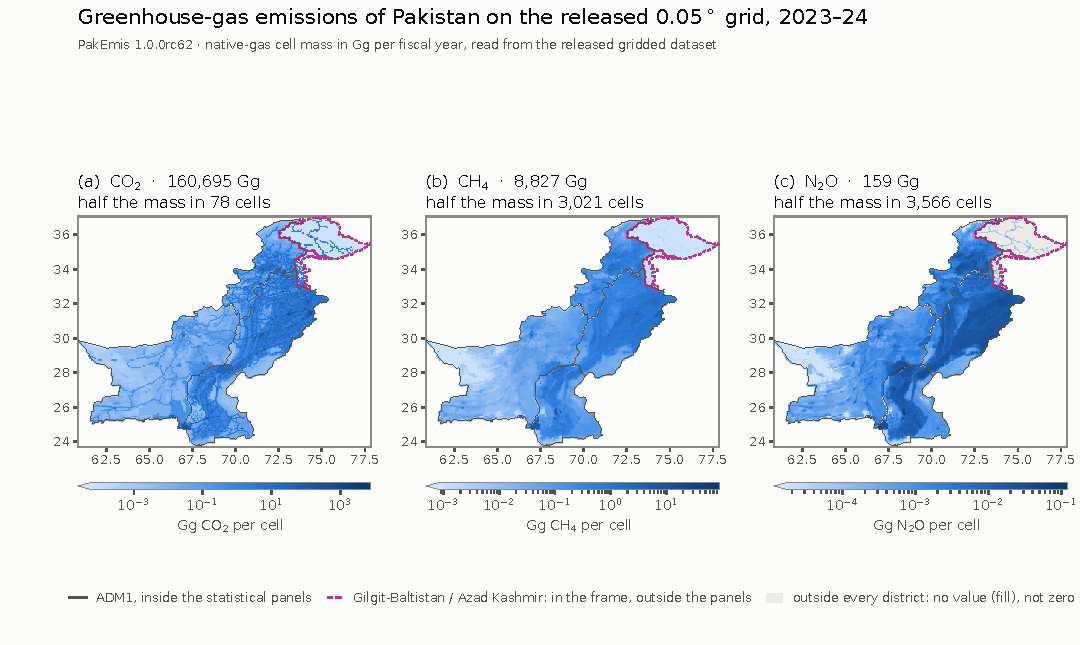
\includegraphics[width=\textwidth,height=0.72\textheight,keepaspectratio]{../../figures/fig_ghg_grid.pdf}
\caption{The released \SI{0.05}{\degree} annual grid for 2023--24. (a--c) Cell totals in native-gas mass for CO$_2$, CH$_4$ and N$_2$O. Each value is the mass emitted in the cell over the fiscal year in Gg of the native gas; values are not normalised by cell area, so they are not a flux density, and cells outside every district carry no value rather than a zero. The subtitle of each panel gives the number of highest-mass cells that hold half of that gas. The evidence behind the placement is shown in Fig.~\ref{fig:grid_evidence}; the companion CSV files carry the plotted values.}
\label{fig:grid}
\end{figure*}

\begin{figure*}[t]
\centering
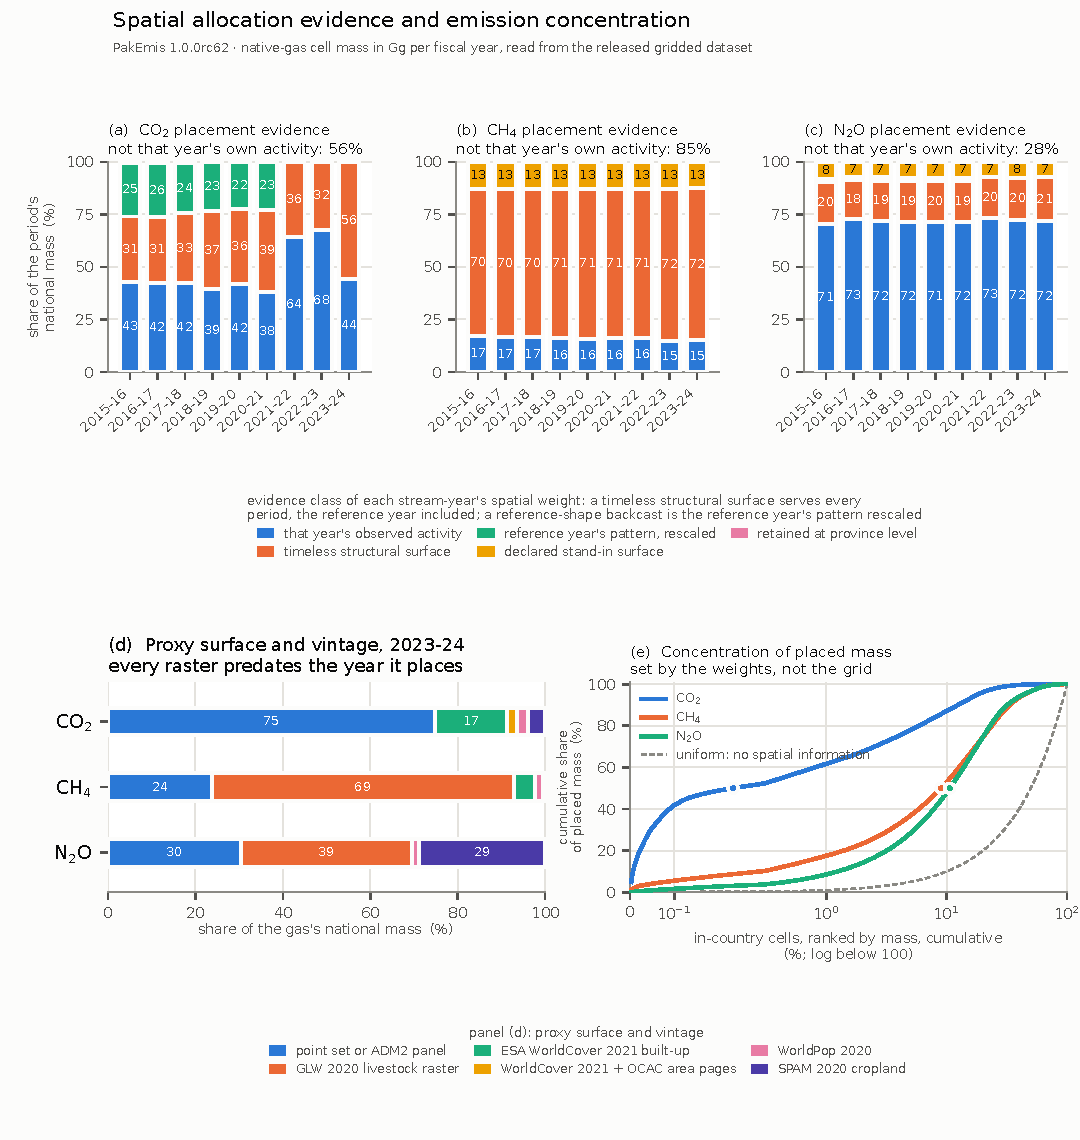
\includegraphics[width=\textwidth,height=0.72\textheight,keepaspectratio]{../../figures/fig_ghg_grid_evidence.pdf}
\caption{Spatial allocation evidence and emission concentration. (a--c) The evidence class behind each period's spatial weight for CO$_2$, CH$_4$ and N$_2$O over the nine periods, as shares of each period's national mass. (d) The proxy surface and its vintage carrying the reference year's mass; every raster predates the fiscal year it places. (e) Concentration: the cumulative share of each gas's placed mass against in-country cells ranked by mass, with the uniform case for reference and a marker at the half-mass point of each curve. The curves are set by the spatial weights, not by the grid, so a finer raster would add no information.}
\label{fig:grid_evidence}
\end{figure*}

\subsection{Sensitivity to source interpretation}
\label{sec:sensitivity}

\paragraph{Household dung.} Using the survey-observed household consumption (configuration S) instead of the agricultural diversion (configuration L) changes residential emissions from \SI{29.47}{\mega\tonne} to \SI{24.33}{\mega\tonne} and the national total from \SI{451.86}{} to \SI{446.73}{\mega\tonne}.

\paragraph{Public-power coal energy.} Four readings of the same stations' coal are carried, differing in calorific basis and coverage. The reference --- station tonnage at the rank-default net calorific value --- gives \SI{40.04}{\mega\tonne} for public power. Station tonnage at the calorific value implied by each station's own heat rate and generation gives \SI{38.45}{\mega\tonne}. The reference with coverage extended to K-Electric gives \SI{44.05}{\mega\tonne}. The regulator's aggregate ``fuel consumed'' energy, which earlier releases used, gives \SI{57.82}{\mega\tonne}; it is retained as a published comparator because it fails the supply bound in Sect.~\ref{sec:coal}. The corresponding national totals are \SI{450.27}{}, \SI{451.86}{}, \SI{455.87}{} and \SI{469.64}{\mega\tonne}. Agreement with an external total cannot select among them, because the readings differ in fuel properties and system coverage rather than in emissions physics.

\paragraph{Sewer conditions and fugitive practice.} Changing the sewer methane correction factor from \num{0.5} to \num{0.1} lowers domestic wastewater from \SI{24.92}{} to \SI{15.85}{\mega\tonne}. Oil and gas fugitive practice and coverage configurations span \SIrange{9.601}{24.694}{\mega\tonne}, with the reference at the upper end. None of these alternatives carries a probability, and they are not combined into one interval.

\paragraph{A parameter endpoint, kept separate.} Raising the wastewater effluent N$_2$O factor from \num{0.005} to \num{0.25}~kg N$_2$O--N per kilogram of nitrogen increases the national total by approximately \SI{148.6}{\mega\tonne}. That range is already sampled in the waste uncertainty specification, so the endpoint is a stress test of a parameter the ensemble represents; it is not a structural alternative and not an additional national upper bound.

\section{Technical validation}
\label{sec:validation}

\subsection{Transcription and date alignment of monthly records}

Monthly reconstruction checks establish that the records were transcribed and dated correctly; they do not independently establish when fuel was burned. Across four OCAC customer classes and three fiscal years, \num{132} of \num{144} reconstructed monthly values agree with separately printed values to the tonne, the maximum difference being \SI{0.14}{\percent}, and an injected one-month displacement is detected in \num{141} cases. Cement dispatches and the PBS production profile differ by a mean of \num{0.22} percentage points of annual activity across \num{60} months, which supports the seasonal shape while keeping sales and production distinct.

\subsection{Comparison with Pakistan's own submission and with EDGAR}
\label{sec:btr}

The most direct comparison is with Pakistan's First Biennial Transparency Report, because its inventory year 2020--21 is a Pakistani fiscal year by its own statement and it reports on AR5 GWPs, so no calendar blend and no GWP-family conversion is needed (Fig.~\ref{fig:validation}). On the \num{16} categories both inventories estimate on a like-for-like boundary, the totals agree to \num{1.02}; the ratio of the two totals excluding LULUCF is \num{1.008}. \num{10} categories lie within a factor of two of the submission and six do not: open burning of waste (\num{17.74}) and oil and gas fugitives (\num{7.27}) above the band; managed soils (\num{0.44}), solid-waste disposal (\num{0.49}), lubricant use (\num{0.43}) and indirect manure N$_2$O (\num{0.37}) below it. Enteric fermentation is \num{1.19} times the submitted value while manure management from the same herd is \num{0.99}; by species, dairy cattle, goats, sheep and camels agree to the submission's printed precision and the difference sits in buffalo and other cattle (\texttt{pakemis\_enteric\_btr\_bridge.csv}). One convention remains unmatched: this inventory weights fossil CH$_4$ at AR5's \num{30} and biogenic CH$_4$ at \num{28}, whereas the submission prints CO$_2$e without a fossil split, so each ratio is also published at a uniform \num{28}, under which the fugitives ratio becomes \num{6.80} and the national ratio \num{1.004}. \num{14} further subjects cannot be expressed as ratios because one side is not estimated, is zero, is booked elsewhere or is a wider aggregate; they are listed in Table~\ref{tab:btr_qualified}.

%% GENERATED by scripts/make_btr_qualified_table.py from btr_qualified_rows.csv. Do not edit.
\begin{table}[t]
\caption{Subjects of the comparison with Pakistan's First Biennial Transparency Report (inventory year 2020--21) that cannot be expressed as a ratio, with the mass each side reports in Mt CO$_2$e (AR5). A blank cell means the account does not estimate the subject.}
\label{tab:btr_qualified}
\footnotesize
\begin{tabular}{@{}>{\raggedright\arraybackslash}p{3.0cm}rr>{\raggedright\arraybackslash}p{3.1cm}@{}}
\tophline
Subject & BTR & PakEmis & Why not a ratio \\
\middlehline
Residue burning, against the submission's cropland non-CO$_2$ & 3.16 & 0.58 & submission carries it only inside a wider aggregate \\
Solid-waste fate (disposal + burning) & 17.83 & 12.08 & submission carries it only inside a wider aggregate \\
Other sectors & 36.80 & 29.64 & scope differs between the two accounts \\
Glass production & 0.03 & -- & estimated only by the submission \\
Industrial wastewater & 2.22 & -- & estimated only by the submission \\
Lime production & 1.33 & -- & estimated only by the submission \\
Other industrial processes & 1.35 & -- & estimated only by the submission \\
Other process uses of carbonates & 0.27 & -- & estimated only by the submission \\
Solid-fuel fugitives & 0.73 & -- & estimated only by the submission \\
Waste incineration & 0.11 & -- & estimated only by the submission \\
Metal industry & 0.00 & 0.38 & reported as zero by the submission \\
ODS substitutes (F-gases) & 0.00 & -- & reported as zero by the submission \\
Field burning of residues & -- & 0.58 & booked under another category by the submission \\
Land (LULUCF) & 34.82 & -- & outside this inventory's scope \\
\bottomhline
\end{tabular}
\end{table}


EDGAR provides a calendar-year comparator across more sectors \citep{EDGAR2025}. Electricity and residential emissions are \num{0.70} and \num{0.94} of EDGAR's calendar-2024 estimates, with the fiscal--calendar offset retained. Industrial combustion is \SI{28.13}{\mega\tonne}~CO$_2$e against \SI{43.98}{\mega\tonne} in EDGAR; both accounts represent the activity, their difference changes sign in earlier years, and the two can share upstream energy statistics, so the \SI{15.85}{\mega\tonne} difference cannot be assigned to missing emissions. The \SI{11.54}{\mega\tonne} EDGAR estimate for fluorinated gases, by contrast, concerns a category PakEmis does not estimate. A transport ratio is withheld because road transport plus mixed off-road machinery does not match EDGAR's multimodal boundary.

Railways provide a matched-year comparison with the earlier submission. The First Biennial Update Report gives \SI{4.06}{\mega\tonne}~CO$_2$e for FY2017--18 \citep{PakistanBUR2022}; the PakEmis method applied to the operator's \num{156396}~thousand litres of diesel for that year gives \SI{0.4664}{\mega\tonne}~CO$_2$e, a factor of \num{8.7} lower, and 2023--24 consumption of \num{132588}~thousand litres gives \SI{0.394}{\mega\tonne}. The \SI{18}{\percent} change in reported consumption between the two years cannot explain the discrepancy, and the Common Reporting Tables' \SI{56609}{\tera\joule} of railway activity for calendar 2022 points to the original activity and factor cells as the place to look \citep{PakistanCRT2026}.

\subsection{The coal supply bound}
\label{sec:coal}

Under the stated coal-rank and calorific assumptions, the aggregate energy estimate requires more coal than reported annual imports and production. Expressed as coal at the generating fleet's own rank composition, the regulator's aggregate energy for 2023--24 requires \SI{29.53}{\mega\tonne} of coal against the \SI{24.72}{\mega\tonne} the national accounts report as imports plus production, \SI{119.5}{\percent} of the supply before any coal reaches a cement plant, a brick kiln or a household. Five tests ask whether the records could reverse this: a supply figure that understates the same twelve months, an inventory drawdown, the assumed lignite share, the coverage of the consumer allocation, and the calorific basis. Each is reported with the change in the records it would require, in the technical supplement; under the stated assumptions none reverses the bound. The station account used for the reference requires \SI{15.88}{\mega\tonne} in the same year, \SI{64}{\percent} of the supply and below the \SI{19.20}{\mega\tonne} the energy yearbook assigns to electricity generation. The aggregate account also implies fleet efficiencies of \SI{57.5}{\percent} in 2020--21 and \SI{18.9}{\percent} in 2023--24, against \SIrange{32.4}{45.7}{\percent} under the generation-implied (heat-rate) calorific basis. The supply bound and the efficiency band are the grounds for preferring the station account; the calorific basis on which the two station readings still differ is treated in the technical documentation. Close offsets between the power and industrial coal allocations indicate dependence within the national coal balance, not independent confirmation of changes in industrial fuel use.

\subsection{Attribution of the managed-soils difference}
\label{sec:soils}

Managed soils contribute \SI{28.53}{\mega\tonne}~CO$_2$e in PakEmis and \SI{58.50}{\mega\tonne} in FAOSTAT, which reports calendar 2023 against our 2023--24 \citep{FAOSTAT2025}. Synthetic-fertiliser nitrogen inputs agree within \SI{0.9}{\percent}, as do the combined counts of six common livestock species, so the input scales are similar and the difference lies in the nitrogen pathways and their factors. Pasture deposition contributes \SI{7.71}{\mega\tonne} here against \SI{27.29}{\mega\tonne} in FAOSTAT, \SI{65.3}{\percent} of the overall difference. Replacing the reference dry-climate EF$_1$ of \num{0.005} with the 2006 aggregate value of \num{0.010} raises managed soils to \SI{40.43}{\mega\tonne}, and applying the earlier pasture-deposition factors as well raises it to \SI{54.72}{\mega\tonne} (Fig.~\ref{fig:soils}); together the two substitutions account for \SI{26.19}{\mega\tonne}, approximately \SI{87}{\percent} of the \SI{29.97}{\mega\tonne} difference, and the remaining \SI{3.78}{\mega\tonne} lies in the indirect factors and nitrogen partitioning. The substitutions apply to distinct nitrogen pathways and are alternative factor choices, not calibration steps: agreement with FAOSTAT does not identify the factors appropriate to Pakistan, and evidence for a dry-climate factor on irrigated cropland does not validate the corresponding treatment of grazing land \citep{IPCC2019}.

\subsection{Facility locations and historical allocation}
\label{sec:locations}

An audit of \num{77} located power stations identifies seven provincial assignments inconsistent with curated or source records, all within \SI{3.4}{\kilo\metre} of a district boundary and representing \SIrange{1.5}{10.3}{\percent} of plant-ledger generation across the audited years; four also disagree with simplified district polygons, so a finer raster alone would not resolve them. The district allocation takes the curated record where one exists, placing a station whose grid cell lies outside its province in the cells of the district its record names, intersected with that province. Across the nine periods this moves between \num{36} and \num{109} districts' allocations in a period and \SIrange{2.4}{20.2}{\mega\tonne} of gross mass in CO$_2$e (AR5), with a net change of order \num{1e-8}~Mt: it is a reallocation within provinces, and no provincial or national total changes.

The provincial split itself is a stated limitation. Each grid fuel carries one provincial share vector, measured on the reference year from the station fuel ledger joined to the curated locations and weighted by energy, and all nine periods reuse it; the stations placed within a province are each period's own, but the share between provinces is the reference year's. For coal, the released exposure table (\texttt{pakemis\_power\_fixed\_pattern\_exposure.csv}) shows that no station carries coal outside its commissioning window, and that on the energy basis the fixed provincial vector differs from each period's own station pool by up to \SI{11.6}{\mega\tonne} in a single province-year before 2022--23 and by at most \SI{0.17}{\mega\tonne} in the reference year. A per-year provincial split is possible in principle from the same records and is a declared revision, not a correction applied here. The provincial comparison of SO$_2$ against EDGAR, which exposes the same limitation from the air-pollutant side, is given in Appendix~\ref{app:so2}.

\begin{figure*}[t]
\centering
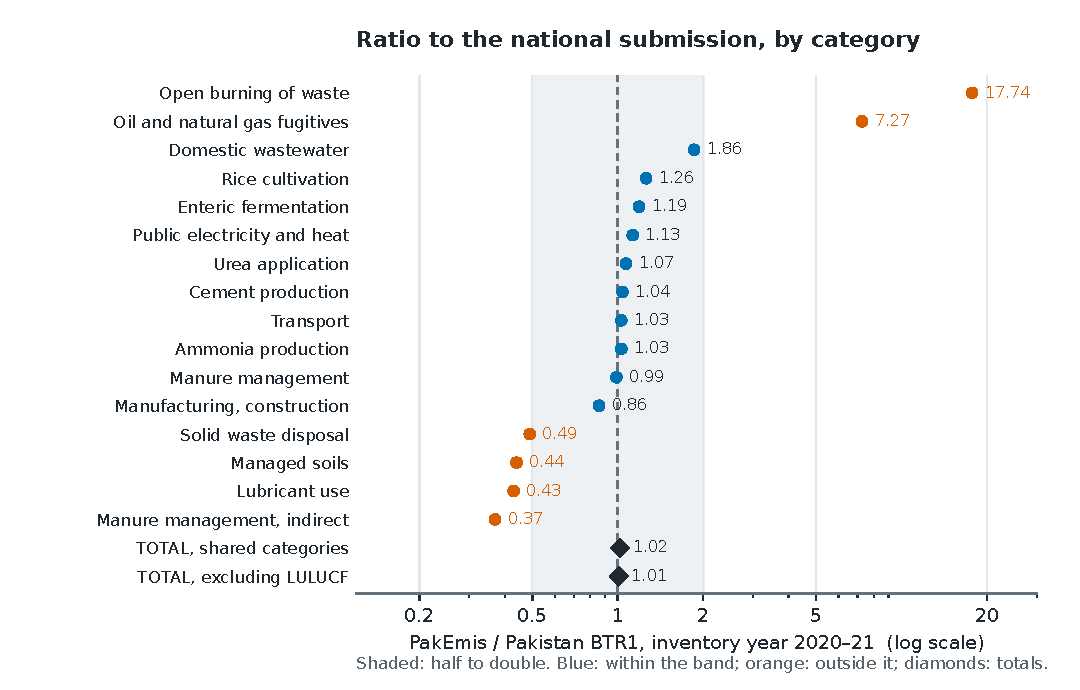
\includegraphics[width=\textwidth,height=0.60\textheight,keepaspectratio]{../../figures/fig4_validation.pdf}
\caption{Comparison with Pakistan's First Biennial Transparency Report, inventory year 2020--21, on AR5 GWPs. Each point is the ratio of the PakEmis estimate to the submitted value for a category both inventories estimate on a like-for-like boundary; totals are shown as diamonds. Shading marks the half-to-double band. Ratios are plotted as published; the alternative weighting of fossil CH$_4$ at \num{28} is given in the product. Subjects that cannot be expressed as a ratio are listed in Table~\ref{tab:btr_qualified}.}
\label{fig:validation}
\end{figure*}

\begin{figure}[t]
\centering
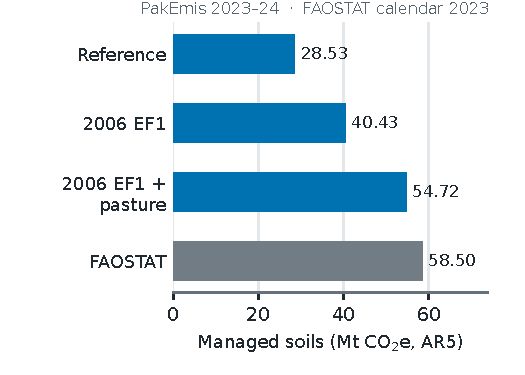
\includegraphics[width=\columnwidth]{../../figures/fig5_managed_soils.pdf}
\caption{Managed-soils N$_2$O under the reference factors and two factor substitutions, beside FAOSTAT. PakEmis describes 2023--24 and FAOSTAT calendar 2023. The substitutions change factors on distinct nitrogen pathways and are not calibration steps.}
\label{fig:soils}
\end{figure}

\section{Data products and recommended use}
\label{sec:use}

Users receive five families of products (Table~\ref{tab:products}): national annual and monthly tables by IPCC category and gas, provincial and district tables, an annual \SI{0.05}{\degree} grid for each of the nine years, a monthly grid for the reference year, and the uncertainty ensemble with the named alternative configurations. Every table carries the category, gas, period, configuration and notation status, and every placement carries its evidence class, so a user can select the detail a question supports.

\begin{table*}[t]
\caption{Core product coverage. Annual and monthly availability refer to the reference configuration; alternative configurations carry their own product identifiers.}
\label{tab:products}
\small
\begin{tabular}{p{0.25\textwidth}p{0.27\textwidth}p{0.38\textwidth}}
\tophline
Product & Period and resolution & Main qualification \\
\middlehline
National tables & Nine fiscal years, annual and monthly & Unestimated categories and the timing evidence class are explicit. \\
Administrative tables & Annual province and district estimates & Fixed boundary frame; historical allocations partly reconstructed. \\
Annual grid & Nine fiscal years, \SI{0.05}{\degree} & Native-gas mass with allocation provenance and an unallocated companion. \\
Monthly grid & 2023--24, \SI{0.05}{\degree} & Combines source timing and location assumptions. \\
Uncertainty and alternatives & Reference ensemble; historical changes; named configurations & Parameter intervals and structural alternatives answer different questions. \\
\bottomhline
\end{tabular}
\end{table*}

How the products should be read follows from how they were built. National annual estimates are the best supported. Monthly values in a category governed by a flat profile express the annual estimate spread by days, not observed seasonality. Historical grids using a fixed or borrowed spatial pattern represent changes in the annual source estimate under that pattern. They should not be interpreted as observations of changing local activity. Near administrative boundaries, a station's provincial assignment can shift district totals, and the provincial split of grid fuels is the reference year's in every period (Sect.~\ref{sec:locations}). A grid-based analysis should retain the unallocated term and use the stated cell-mass convention. A comparison with another inventory should first match the emitting sources, the period and the gas metric.

Four source questions remain open, each with the size of what it would move. Managed soils is the largest: the reference estimates \SI{28.53}{\mega\tonne}\,CO$_2$e for 2023--24, two factor substitutions inside the same method give \SI{40.43}{} and \SI{54.72}{\mega\tonne}, and FAOSTAT reports \SI{58.50}{\mega\tonne}. The livestock bridge is next: enteric fermentation is \SI{58.0}{\percent} of the Approach~1 variance screen, and against the submission for FY2020--21 it is \num{1.19} times the submitted value while manure management from the same herd is \num{0.99} times, with the difference confined to buffalo and other cattle. Crop residues are \num{0.18} of the submission's cropland non-CO$_2$ line, which is a wider aggregate than the inventory's own row. Solid waste is a specification question: disposal is \num{0.49} of the submitted figure and the broader fate account \num{0.68}. None of the four is settled by evidence this release holds, and none receives a provisional correction; each needs activity or factor evidence that we have not acquired or reconciled (\texttt{data/shared/requests/data\_gaps.csv}).

Reproducibility has two levels. The calculation can be rebuilt from the compiled activity tables with the released software, and the test suite checks the identities between the products. Re-deriving a compiled table from its primary document is possible only where the document is held: some cited primary documents have not been retained, and some held validation products have only partial re-derivation checks. File checksums establish which release a number came from; they do not show that a source transcription was correct. The technical documentation lists each product's reproduction level.

\FloatBarrier
\conclusions

PakEmis combines publicly available activity statistics with IPCC methods and reconciles fuel and biomass quantities shared between sectors. It links annual estimates to monthly and spatial products while recording the evidence supporting their allocation. The reference-year total is \SI{451.86}{\mega\tonne}~CO$_2$e on the AR5 basis, with a conditional parameter interval of \SIrange{406.71}{532.86}{\mega\tonne}; the estimated increase of \SI{50.96}{\mega\tonne} over the study period excludes zero under the reference and time-correlated dependence settings and includes it under time independence (\SIrange{-12.48}{117.11}{\mega\tonne}). Methane is \SI{55.1}{\percent} of the total and enteric fermentation a third of it, so the livestock series and its factors govern both the level and its uncertainty.

Three limitations matter most for interpretation. The public-power coal account rests on the stations' metered tonnage because the regulator's aggregate energy exceeds the national coal supply; the calorific basis of that tonnage is still an open choice worth \SI{1.6}{\mega\tonne}. The household dung quantity is read two ways that differ by \SI{5.1}{\mega\tonne} nationally, and the evidence held does not decide between them. The monthly and spatial products carry their annual estimates on profiles and patterns that are, for most of the mass, not observations of that year, and the evidence class attached to each placement is the guide to what they support.

\dataavailability{The dataset is PakEmis version 1.0.0rc62 (the release candidate this manuscript describes). The released products, their checksums (\texttt{outputs/SHA256SUMS}) and the release manifest naming the repository commit are archived with the software; the dataset DOI, the review link and the version-specific citation are pending registration of the deposit and will be inserted here.}

\codeavailability{The source code is at \url{https://github.com/RehanAhmad13/pakistan-emissions-sectors}; the commit the release describes is recorded in \texttt{outputs/release\_manifest.json}. Reproduction is documented in \texttt{docs/reproducibility.md}: the inventory rebuilds with \texttt{python3 -m pkinv.run\_all} and the test suite runs with \texttt{python3 -m unittest discover -s tests}. The software archive identifier is pending with the dataset DOI.}

\authorcontribution{RA designed the inventory, compiled the source data, developed the calculation software and tests, produced the data records and wrote the paper.}
\competinginterests{The author declares no competing interests.}

% Release provenance: generated from outputs/release_manifest.json by
% scripts/make_release_cover.py; placed after the availability statements so that dataset
% identity is where ESSD readers look for it and hashes stay out of the front matter.
%% GENERATED by scripts/make_release_cover.py from outputs/release_manifest.json.
%% Do not edit: the edit will be overwritten and CI diffs the result.
\newcommand{\ReleaseCover}{%
\begin{center}\small
\setlength{\fboxsep}{4pt}%
\fbox{\begin{minipage}{\dimexpr\linewidth-2\fboxsep-2\fboxrule\relax}\footnotesize
\textbf{Release provenance.} This document describes PakEmis under the period, configuration and source boundaries specified in its methods. The identifiers below link it to the accompanying products and source register.\\[2pt]
\begin{tabular}{@{}p{0.32\linewidth}@{\hspace{0.03\linewidth}}p{0.65\linewidth}@{}}
Release version & \texttt{1.0.0rc69} \\
Commit & \texttt{d8d874622f9a} \\
Reporting period & July 2015--June 2025 (ten fiscal years) (2015-07-01 to 2025-06-30) \\
Reference & S\_TAN (household survey; TAN nitrogen) \\
FY2023--24 total & 444.61 Mt \COe{} (AR5) under S\_TAN, the reference; 449.85 Mt under L\_TAN \\
Release manifest & \texttt{ac0ffe93ad9fcd88} (SHA-256 of \texttt{outputs/release\_manifest.json}, first 16) \\
Source manifest & \texttt{c1be6d314cfce1ea} (SHA-256 of \texttt{data/manifests/source\_manifest.csv}, first 16) \\
Data-description article & \texttt{paper\_national/} (ESSD, in preparation), same release
\end{tabular}
\end{minipage}}
\end{center}}

\ReleaseCover

\appendix
\section{Provincial sulphur dioxide against EDGAR}
\label{app:so2}

Provincial SO$_2$ reveals differences that national aggregation conceals. EDGAR v8.1 emissions are integrated into common administrative boundaries using fractional grid-cell areas, with adjacent calendar years blended for the fiscal comparison \citep{EDGARAP81}. For FY2021--22 the national PakEmis-to-EDGAR ratio is \num{0.96}, but the provincial ratios are \num{1.30} in Punjab, \num{1.72} in Khyber Pakhtunkhwa, \num{2.06} in Balochistan and \num{0.21} in Sindh (\texttt{pakemis\_air\_provincial\_external\_comparison.csv}); opposing provincial differences nearly cancel nationally. Neither inventory supplies observed provincial emissions against which these ratios could be read as accuracy scores.

Electricity generation is the principal source of the disagreement: the PakEmis power layer gives \SI{167.0}{\giga\gram} against EDGAR's \SI{409.3}{\giga\gram}, including \SI{4.5}{} against \SI{196.9}{\giga\gram} in Sindh. The PakEmis layer includes oil and diesel; coal SO$_2$ is a separate screening calculation because desulphurisation performance is unresolved. Adding the coal-screening estimates gives \SI{202.0}{\giga\gram} under the controlled case and \SI{362.2}{\giga\gram} under the uncontrolled case, so EDGAR lies above the screening range, exceeding its uncontrolled endpoint by \SI{47.1}{\giga\gram} (\SI{13}{\percent}). This identifies a consequential coverage and control assumption without establishing that plants operate without effective desulphurisation.

\begin{thebibliography}{99}

\bibitem[Climate TRACE(2026)]{ClimateTRACE2026}
Climate TRACE: Climate TRACE Emissions Inventory and Data Downloads, country- and source-level records accessed through API v7 on 6 August 2026, \url{https://climatetrace.org/data}, 2026.

\bibitem[Crippa et~al.(2025)]{EDGAR2025}
Crippa, M., Guizzardi, D., Pagani, F., Banja, M., Muntean, M., Schaaf, E., Quadrelli, R., Risquez Martin, A., Taghavi-Moharamli, P., K\"oykk\"a, J., Grassi, G., Rossi, S., Melo, J., Jacome Felix Oom, D., Branco, A., Su\'arez-Moreno, M., Sedano, F., San-Miguel, J., Manca, G., Pisoni, E., and Pekar, F.: GHG emissions of all world countries---2025 report, JRC143227, Publications Office of the European Union, Luxembourg, \doi{10.2760/9816914}, 2025.

\bibitem[Crippa et~al.(2026)]{EDGARAP81}
Crippa, M., Guizzardi, D., Pagani, F., Banja, M., Muntean, M., Schaaf, E., Becker, W., Monforti Ferrario, F., Quadrelli, R., Risquez Martin, A., Grassi, G., Rossi, S., Brandao De Melo, J., Jacome Felix Oom, D., Branco, A., San-Miguel, J., and Vignati, E.: EDGAR v8.1 Global Air Pollutant Emissions, European Commission, Joint Research Centre [data set], \doi{10.2905/JRC.E1ZGQER}, 2026.

\bibitem[FAO(2025)]{FAOSTAT2025}
FAO: FAOSTAT: emissions totals, crops and livestock, fertilisers by nutrient, and forestry production and trade, Food and Agriculture Organization of the United Nations, Rome [data sets], \url{https://www.fao.org/faostat/}, 2025 snapshot used in the source inventory; catalogue checked 30 September 2026, 2025.

\bibitem[Government of Pakistan(2022)]{PakistanBUR2022}
Government of Pakistan: Pakistan's First Biennial Update Report to the United Nations Framework Convention on Climate Change, Ministry of Climate Change, Islamabad, \url{https://unfccc.int/documents/470405}, 2022.

\bibitem[Government of Pakistan(2024)]{PakistanBTR2024}
Government of Pakistan: Pakistan's First Biennial Transparency Report to the UNFCCC, Ministry of Climate Change and Environmental Coordination, \url{https://unfccc.int/documents/645241}, report designated 2024; UNFCCC landing page published 16 June 2025, 2024.

\bibitem[Government of Pakistan(2026)]{PakistanCRT2026}
Government of Pakistan: Pakistan: 2024 Common Reporting Table (CRT), UNFCCC submission, \url{https://unfccc.int/documents/655653}, submitted 6 February 2026, 2026.

\bibitem[IPCC(2006)]{IPCC2006}
IPCC: 2006 IPCC Guidelines for National Greenhouse Gas Inventories, edited by: Eggleston, H. S., Buendia, L., Miwa, K., Ngara, T., and Tanabe, K., Institute for Global Environmental Strategies, Hayama, Japan, \url{https://www.ipcc-nggip.iges.or.jp/public/2006gl/}, 2006.

\bibitem[IPCC(2013)]{IPCCAR5}
IPCC: Climate Change 2013: The Physical Science Basis, Cambridge University Press, Cambridge, \doi{10.1017/CBO9781107415324}, 2013.

\bibitem[IPCC(2019)]{IPCC2019}
IPCC: 2019 Refinement to the 2006 IPCC Guidelines for National Greenhouse Gas Inventories, edited by: Calvo Buendia, E., Tanabe, K., Kranjc, A., Baasansuren, J., Fukuda, M., Ngarize, S., Osako, A., Pyrozhenko, Y., Shermanau, P., and Federici, S., IPCC, Switzerland, \url{https://www.ipcc-nggip.iges.or.jp/public/2019rf/}, 2019.

\bibitem[IPCC(2021)]{IPCCAR6}
IPCC: Climate Change 2021: The Physical Science Basis, Cambridge University Press, Cambridge, \doi{10.1017/9781009157896}, 2021.

\bibitem[PBS(2026a)]{PBSAgri2026}
PBS: Agricultural Census 2024, Pakistan Bureau of Statistics, Islamabad, report collection, \url{https://www.pbs.gov.pk/agriculture-census/}, accessed 30 September 2026, 2026a.

\bibitem[PBS(2026b)]{PBSHIES2026}
PBS: Household Integrated Economic Survey (HIES) 2024--25, Pakistan Bureau of Statistics, Islamabad, \url{https://www.pbs.gov.pk/household-integrated-economic-survey-hies-2024-25/}, accessed 30 September 2026, 2026b.

\bibitem[Tubiello et~al.(2013)]{Tubiello2013}
Tubiello, F. N., Salvatore, M., Rossi, S., Ferrara, A., Fitton, N., and Smith, P.: The FAOSTAT database of greenhouse gas emissions from agriculture, Environmental Research Letters, 8, 015009, \doi{10.1088/1748-9326/8/1/015009}, 2013.

\end{thebibliography}

\end{document}
